\section{Thiết kế dữ liệu}

\begin{figure}[H]
  \centering
  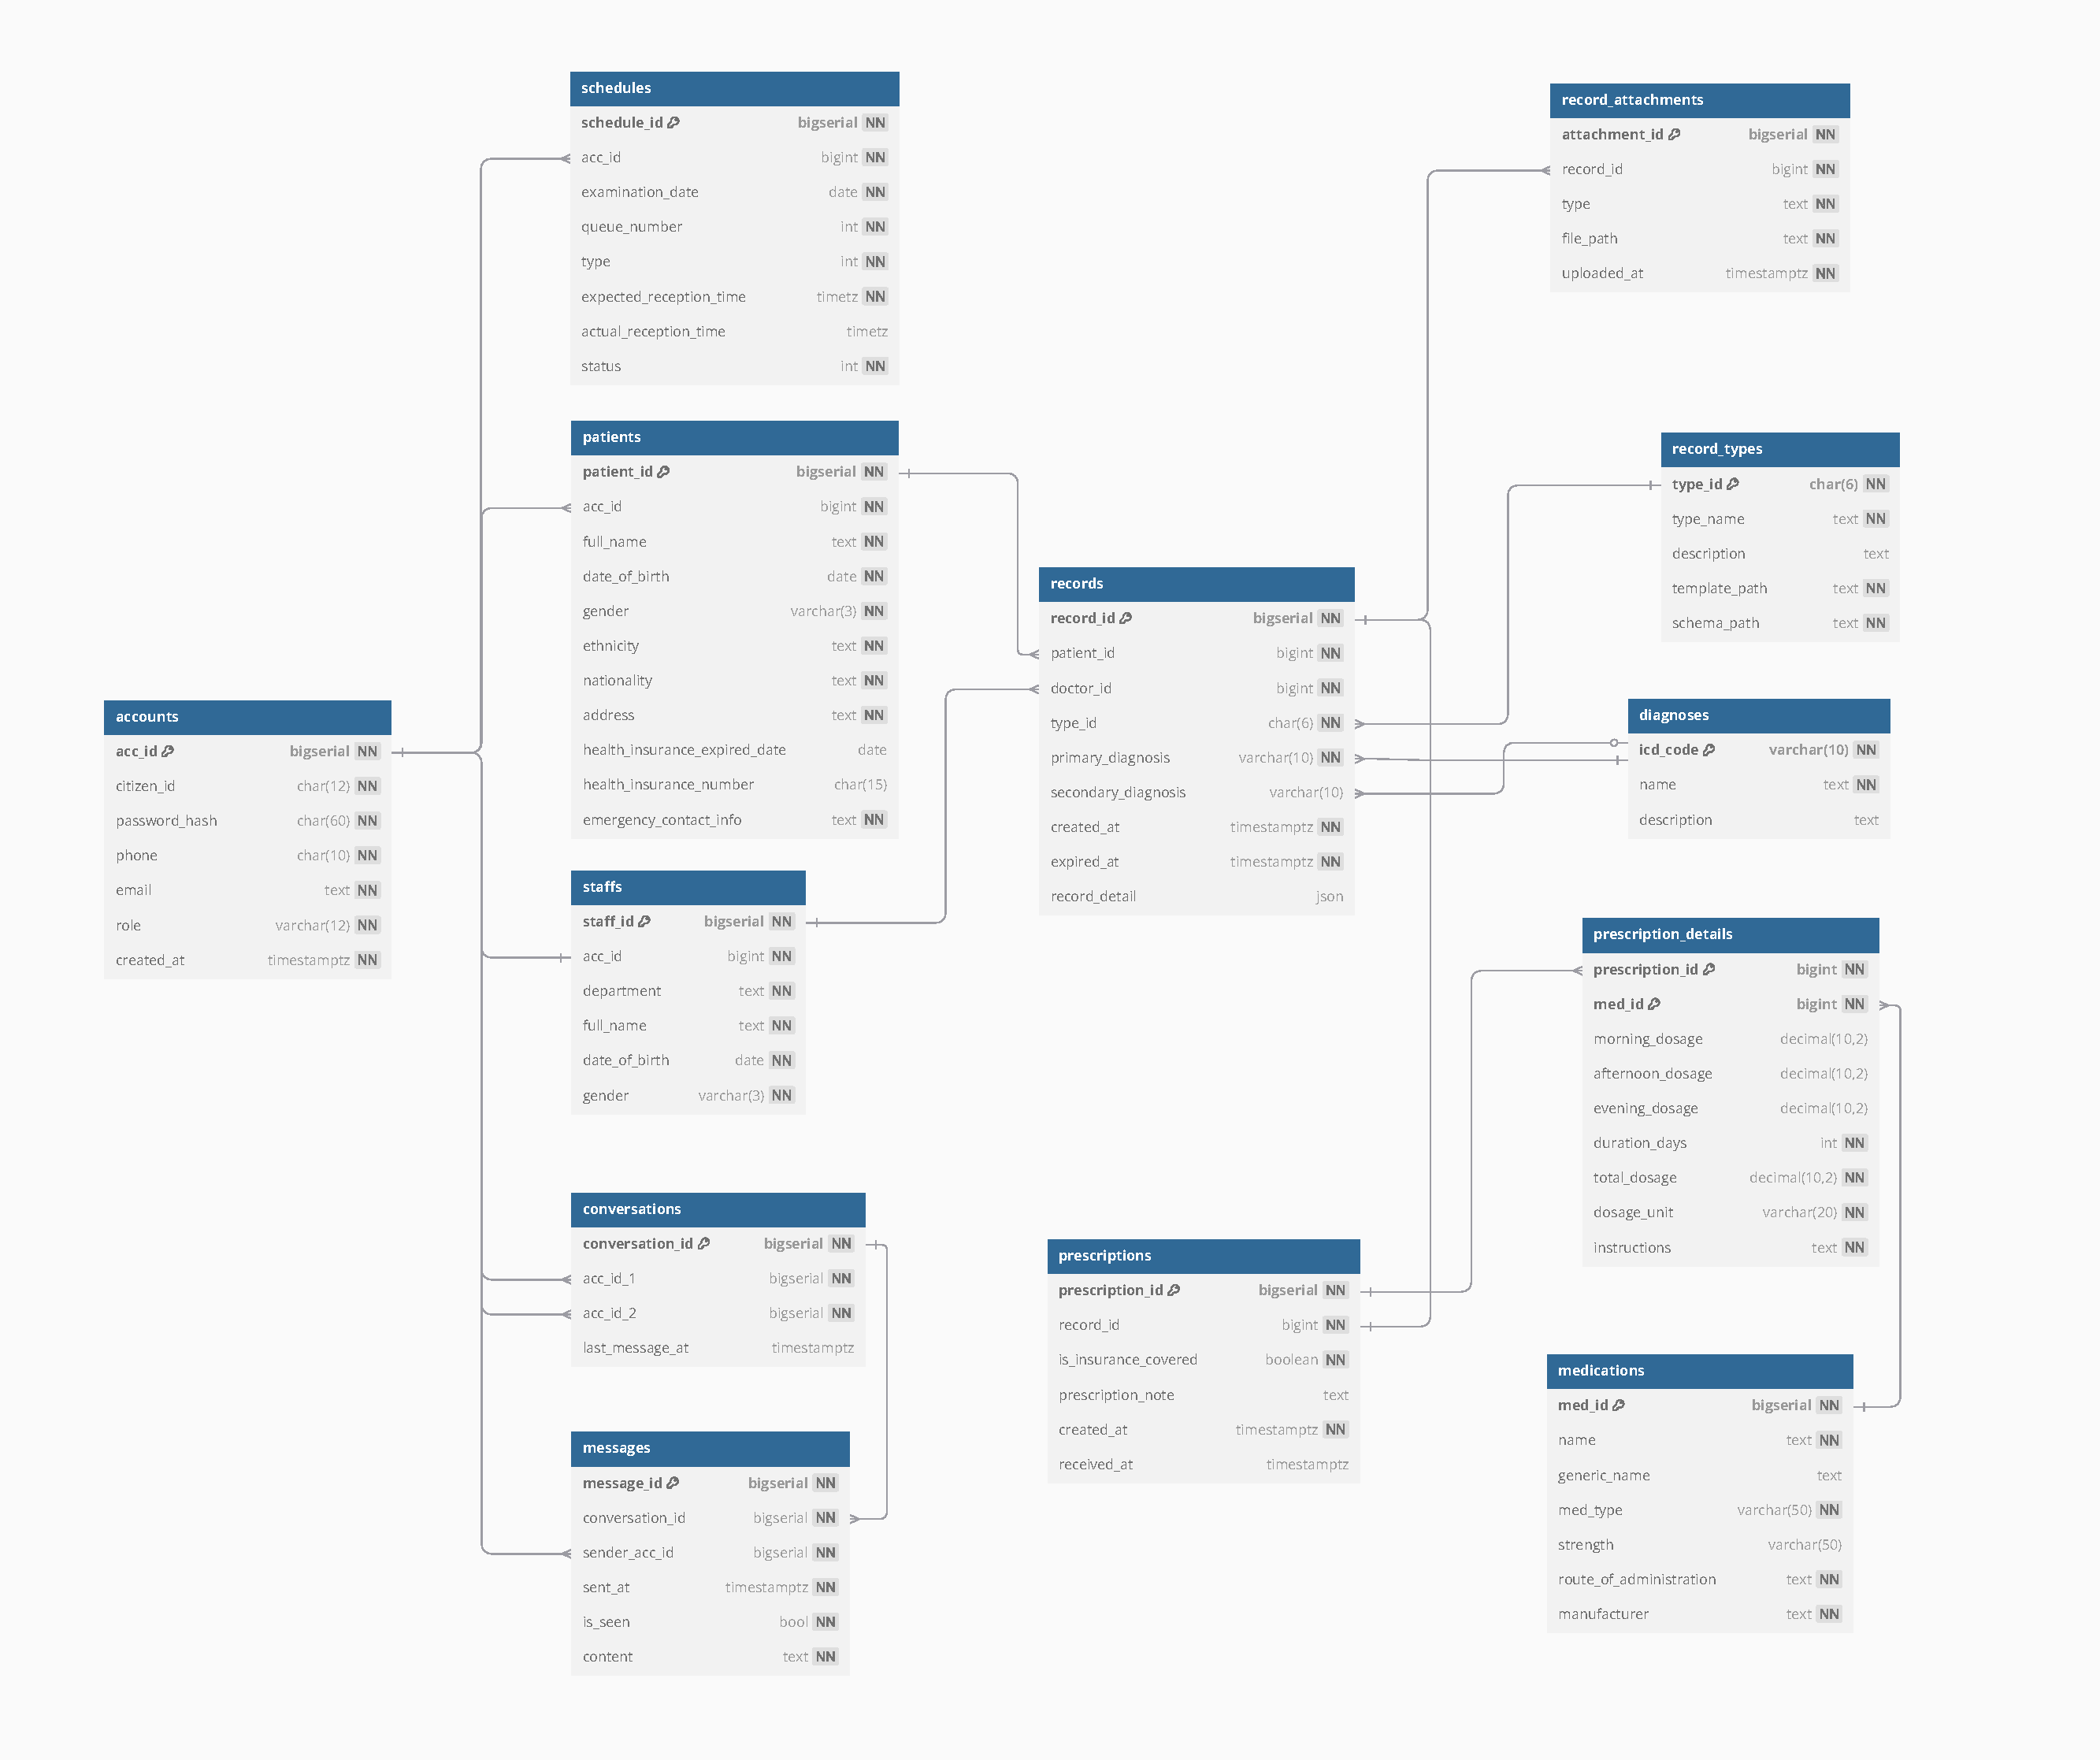
\includegraphics[width=1\textwidth]{src/figures/schema.pdf}
  \caption{Lược đồ cơ sở dữ liệu chính của MeReMa}
  \label{fig:schema}
\end{figure}

\subsection{Bảng accounts}
Bảng \texttt{accounts} lưu trữ thông tin về tài khoản người dùng, bao gồm các trường như:
\begin{itemize}
  \item \texttt{acc\_id} (pk): Mã định danh duy nhất của tài khoản.
  \item \texttt{citizen\_id}: Số CCCD của người dùng, được sử dụng để xác định danh tính tài khoản.
  \item \texttt{password\_hash}: Mật khẩu đã được mã hóa của tài khoản.
  \item \texttt{phone}: Số điện thoại của người dùng, có thể dùng để làm định danh tài khoản.
  \item \texttt{email}: Email của người dùng, có thể dùng để làm định danh tài khoản.
  \item \texttt{role}: Vai trò của tài khoản, bao gồm các vai trò như \texttt{admin}, \texttt{doctor}, \texttt{receptionist} và \texttt{patient}.
  \item \texttt{created\_at}: Ngày giờ tạo tài khoản.
\end{itemize}

\subsection{Bảng staffs}
Bảng \texttt{staffs} lưu thông tin về các nhân viên bệnh viện sử dụng hệ thống.
\begin{itemize}
  \item \texttt{staff\_id} (pk): Mã định danh duy nhất của nhân viên.
  \item \texttt{acc\_id}: Khóa ngoại liên kết với bảng \texttt{accounts}, đảm bảo mỗi nhân viên có một tài khoản duy nhất.
  \item \texttt{department}: Khoa hoặc phòng ban mà nhân viên công tác.
  \item \texttt{full\_name}: Họ tên đầy đủ của nhân viên.
  \item \texttt{date\_of\_birth}: Ngày sinh của nhân viên.
  \item \texttt{gender}: Giới tính của nhân viên.
\end{itemize}

\subsection{Bảng patients}
Bảng \texttt{patients} lưu thông tin cá nhân của bệnh nhân đã và đang thăm khám tại bệnh viện.
\begin{itemize}
  \item \texttt{patient\_id} (pk): Mã định danh duy nhất của bệnh nhân.
  \item \texttt{acc\_id}: Khóa ngoại liên kết với bảng \texttt{accounts}, đại diện cho tài khoản của bệnh nhân.
  \item \texttt{full\_name}: Họ tên đầy đủ của bệnh nhân.
  \item \texttt{date\_of\_birth}: Ngày sinh.
  \item \texttt{gender}: Giới tính.
  \item \texttt{ethnicity}: Dân tộc của bệnh nhân.
  \item \texttt{nationality}: Quốc tịch của bệnh nhân.
  \item \texttt{address}: Địa chỉ thường trú hoặc liên hệ.
  \item \texttt{health\_insurance\_expired\_date}: Ngày hết hạn thẻ bảo hiểm y tế.
  \item \texttt{health\_insurance\_number}: Mã số thẻ bảo hiểm y tế.
  \item \texttt{emergency\_contact\_info}: Thông tin liên lạc khẩn cấp.
\end{itemize}

\subsection{Bảng records}
Bảng \texttt{records} lưu trữ thông tin hồ sơ bệnh án.
\begin{itemize}
  \item \texttt{record\_id} (pk): Mã định danh duy nhất của hồ sơ bệnh án.
  \item \texttt{patient\_id}: Khóa ngoại liên kết với bảng \texttt{patients}.
  \item \texttt{doctor\_id}: Khóa ngoại liên kết với bảng \texttt{staffs}, đại diện cho bác sĩ phụ trách.
  \item \texttt{type\_id}: Khóa ngoại liên kết với bảng \texttt{record\_types}, chỉ loại hồ sơ bệnh án.
  \item \texttt{primary\_diagnosis}: Mã ICD của chẩn đoán chính.
  \item \texttt{secondary\_diagnosis}: Mã ICD của chẩn đoán phụ.
  \item \texttt{created\_at}: Thời điểm tạo hồ sơ.
  \item \texttt{expired\_at}: Thời điểm hết hiệu lực của hồ sơ (mặc định sau 10 năm).
  \item \texttt{record\_detail}: Nội dung chi tiết của hồ sơ bệnh án, lưu ở định dạng JSON.
\end{itemize}

\subsection{Bảng record\_types}
Bảng \texttt{record\_types} định nghĩa các loại hồ sơ bệnh án.
\begin{itemize}
  \item \texttt{type\_id} (pk): Mã loại hồ sơ.
  \item \texttt{type\_name}: Tên hiển thị của loại hồ sơ.
  \item \texttt{description}: Mô tả chi tiết về loại hồ sơ.
  \item \texttt{template\_path}: Đường dẫn đến mẫu hiển thị hồ sơ.
  \item \texttt{schema\_path}: Đường dẫn đến schema JSON dùng để hợp thức hóa chi tiết hồ sơ bệnh án.
\end{itemize}

\subsection{Bảng diagnoses}
Bảng \texttt{diagnoses} lưu danh mục các mã chẩn đoán ICD.
\begin{itemize}
  \item \texttt{icd\_code} (pk): Mã ICD-10.
  \item \texttt{name}: Tên của chẩn đoán.
  \item \texttt{description}: Mô tả chi tiết về chẩn đoán.
\end{itemize}

\subsection{Bảng record\_attachments}
Bảng \texttt{record\_attachments} lưu thông tin các tệp đính kèm của hồ sơ bệnh án.
\begin{itemize}
  \item \texttt{attachment\_id} (pk): Mã định danh của tệp đính kèm.
  \item \texttt{record\_id}: Khóa ngoại liên kết với hồ sơ bệnh án tương ứng.
  \item \texttt{type}: Loại tệp đính kèm (ví dụ: x - quang, siêu âm, ...).
  \item \texttt{file\_path}: Đường dẫn lưu trữ tệp.
  \item \texttt{uploaded\_at}: Thời điểm tệp được tải lên.
\end{itemize}

\subsection{Bảng prescriptions}
Bảng \texttt{prescriptions} lưu thông tin đơn thuốc.
\begin{itemize}
  \item \texttt{prescription\_id} (pk): Mã định danh đơn thuốc.
  \item \texttt{record\_id}: Khóa ngoại liên kết với hồ sơ bệnh án.
  \item \texttt{is\_insurance\_covered}: Cờ đánh dấu đơn thuốc có được BHYT chi trả hay không.
  \item \texttt{prescription\_note}: Ghi chú của bác sĩ về đơn thuốc.
  \item \texttt{created\_at}: Thời điểm tạo đơn thuốc.
  \item \texttt{received\_at}: Thời điểm bệnh nhân nhận thuốc.
\end{itemize}

\subsection{Bảng prescription\_details}
Bảng \texttt{prescription\_details} chứa thông tin chi tiết về các loại thuốc trong một đơn.
\begin{itemize}
  \item \texttt{prescription\_id} (pk): Khóa ngoại liên kết với bảng \texttt{prescriptions}.
  \item \texttt{med\_id} (pk): Khóa ngoại liên kết với bảng \texttt{medications}.
  \item \texttt{morning\_dosage}, \texttt{afternoon\_dosage}, \texttt{evening\_dosage}: Liều dùng vào buổi sáng, chiều, tối.
  \item \texttt{duration\_days}: Số ngày sử dụng thuốc.
  \item \texttt{total\_dosage}: Tổng liều lượng trong đơn.
  \item \texttt{dosage\_unit}: Đơn vị liều dùng (ví dụ: viên, ml...).
  \item \texttt{instructions}: Hướng dẫn sử dụng thuốc.
\end{itemize}

\subsection{Bảng medications}
Bảng \texttt{medications} lưu danh mục các loại thuốc.
\begin{itemize}
  \item \texttt{med\_id} (pk): Mã định danh của thuốc.
  \item \texttt{name}: Tên thương mại của thuốc.
  \item \texttt{generic\_name}: Tên hoạt chất chính (nếu có).
  \item \texttt{med\_type}: Dạng thuốc (viên, nước, tiêm...).
  \item \texttt{strength}: Hàm lượng hoạt chất (ví dụ: 500mg).
  \item \texttt{route\_of\_administration}: Đường dùng (uống, tiêm, bôi...).
  \item \texttt{manufacturer}: Tên nhà sản xuất.
\end{itemize}

\subsection{Bảng conversations}
Bảng \texttt{conversations} lưu thông tin các cuộc hội thoại giữa hai tài khoản.
\begin{itemize}
  \item \texttt{conversation\_id} (pk): Mã định danh của cuộc hội thoại.
  \item \texttt{acc\_id\_1}, \texttt{acc\_id\_2}: Hai tài khoản tham gia cuộc trò chuyện.
  \item \texttt{last\_message\_at}: Thời điểm gửi tin nhắn gần nhất.
\end{itemize}

\subsection{Bảng messages}
Bảng \texttt{messages} lưu các tin nhắn trong cuộc hội thoại.
\begin{itemize}
  \item \texttt{message\_id} (pk): Mã định danh của tin nhắn.
  \item \texttt{conversation\_id}: Khóa ngoại đến bảng \texttt{conversations}.
  \item \texttt{sender\_acc\_id}: Tài khoản gửi tin nhắn.
  \item \texttt{sent\_at}: Thời điểm gửi.
  \item \texttt{is\_seen}: Trạng thái đã đọc của tin nhắn.
  \item \texttt{content}: Nội dung tin nhắn.
\end{itemize}

\subsection{Bảng schedules}
Bảng \texttt{schedules} lưu thông tin lịch khám bệnh.
\begin{itemize}
  \item \texttt{schedule\_id} (pk): Mã định danh của lịch hẹn.
  \item \texttt{acc\_id}: Tài khoản của bệnh nhân đặt lịch.
  \item \texttt{examination\_date}: Ngày khám bệnh.
  \item \texttt{queue\_number}: Số thứ tự trong ngày.
  \item \texttt{type}: Loại khám (\texttt{1} - BHYT, \texttt{2} - dịch vụ).
  \item \texttt{expected\_reception\_time}: Thời gian dự kiến được gọi vào khám.
  \item \texttt{actual\_reception\_time}: Thời gian thực tế được gọi vào khám.
  \item \texttt{status}: Trạng thái của lịch hẹn (\texttt{1} - chờ khám, \texttt{2} - đã khám, \texttt{3} - hủy...).
\end{itemize}